\documentclass[conference]{IEEEtran}
\usepackage{cite}
\usepackage{amsmath,amssymb,amsfonts}
\usepackage{algorithmic}
\usepackage{graphicx}
\usepackage{textcomp}
\usepackage{xcolor}
\usepackage{color} 
\usepackage{listings}
\def\BibTeX{{\rm B\kern-.05em{\sc i\kern-.025em b}\kern-.08em
    T\kern-.1667em\lower.7ex\hbox{E}\kern-.125emX}}
\graphicspath{ {Images/} }

% Python Syntax Styling
\definecolor{Code}{rgb}{0,0,0} 
\definecolor{Decorators}{rgb}{0.5,0.5,0.5} 
\definecolor{Numbers}{rgb}{0.5,0,0} 
\definecolor{MatchingBrackets}{rgb}{0.25,0.5,0.5} 
\definecolor{Keywords}{rgb}{0,0,1} 
\definecolor{self}{rgb}{0,0,0} 
\definecolor{Strings}{rgb}{0,0.63,0} 
\definecolor{Comments}{rgb}{0,0.63,1} 
\definecolor{Backquotes}{rgb}{0,0,0} 
\definecolor{Classname}{rgb}{0,0,0} 
\definecolor{FunctionName}{rgb}{0,0,0} 
\definecolor{Operators}{rgb}{0,0,0} 
\definecolor{Background}{rgb}{0.98,0.98,0.98} 
 
\lstdefinelanguage{Python}{ 
numbers=left, 
numberstyle=\footnotesize, 
numbersep=1em, 
xleftmargin=1em, 
framextopmargin=2em, 
framexbottommargin=2em, 
showspaces=false, 
showtabs=false, 
showstringspaces=false, 
frame=l, 
tabsize=4, 
% Basic 
basicstyle=\ttfamily\small, 
backgroundcolor=\color{Background}, 
% Comments 
commentstyle=\color{Comments}\slshape, 
% Strings 
stringstyle=\color{Strings}, 
morecomment=[s][\color{Strings}]{"""}{"""}, 
morecomment=[s][\color{Strings}]{'''}{'''}, 
% keywords 
morekeywords={import,from,class,def,for,while,if,is,in,elif,else,not,and,or,print,break,continue,return,True,False,None,access,as,,del,except,exec,finally,global,import,lambda,pass,print,raise,try,assert}, 
keywordstyle={\color{Keywords}\bfseries}, 
% additional keywords 
morekeywords={[2]@invariant,pylab,numpy,np,scipy}, 
keywordstyle={[2]\color{Decorators}\slshape}, 
emph={self}, 
emphstyle={\color{self}\slshape}, 
% 
}
% End Python Syntax Styling

\begin{document}

\title{Conference Paper Title}

\author{
\IEEEauthorblockN{Alison Major}
\IEEEauthorblockA{\textit{Computer Science} \\
\textit{Lewis University}\\
Romeoville, Illinois, USA \\
AlisonMMajor@lewisu.edu}
}

\maketitle

\begin{abstract}
Data is found in a variety of digital formats: email messages, spreadsheets, images, sound files. There are a number of tools that have been designed to assist in automatically extract data from certain formats. Optical Character Recognition (known as OCR) can be used to convert images into text, though not always in a structured and useful format. Natural-language processing allows computers to extract information from text written in the natural language form. Is there a way to allow multiple forms of information to be received by a system and automatically pull the desired data from those different formats? For example, if a customer submits a purchase order as a scanned image that we want to automatically pull item numbers from, what is the ideal number of documents needed to "train" that system? Similarly, if a customer submits an order in an email message in prose or with an embedded table, what are our options for extracting the desired information? This paper will review technologies that use OCR, natural-language processing, and machine learning to find optimal options for extracting data from a variety of inputs.
\end{abstract}

\begin{IEEEkeywords}
OCR, RPA
\end{IEEEkeywords}

\section{Introduction}
Many companies receive input from users in a variety of ways. Some may email, some send attached files.

For a human to process these, they need to read the information in whichever format it is received, then understand it enough to enter it into the appropriate system.

In this paper, we'll focus on receiving orders and adding them to a company's ordering system.

In an ideal situation, customer orders will be received in a consistent format. However, when there are a large number of customers, or if some carry a lot of weight, they will stick with the process that is easiest for them. This means that whatever comes out of the systems and applications that they use is what you will need to work from.

There are many solutions already available.

\section{Manual Data Entry}
In 2018, Goldman Sachs reported that the direct and indirect cost of manual data entry for global businesses was estimated to be about \$2.7 trillion \cite{schneider2018b2b}. Gartner's study in 2019 found that avoidable rework in accounting departments amounted to 30\% of a full-time employees' time; for an accounting staff of 40 full-time employees, this amounts to 25,000 hours per year and about \$878,000 \cite{lavelle2019gartner}!

While modern applications provide us with many conveniences, many companies or industries have legacy processes in place. People deal with paper forms and documents every day, which then must be typed into digital systems. This manual data entry leaves room for error, as Gartner found. Additionally, manual entry is very time-consuming.

\section{What is OCR?}
Optical Character Recognition, more commonly known as OCR, is a technique that results in converting images and files into machine-readable data. The technology reviews images for fonts and shapes, matching information with text that can be reviewed and stored.

While providing actionable information, there are still many challenges with OCR. Images and pages may be received with incorrect orientation or skewed at an angle. There may be noise or distortion on the page, or handwriting overlapping the printed text. Background colors or images can impact the technology's ability to get a clear read on the information.

Some of these challenges can be overcome through the use of preprocessing. Pages can be scaled and adjusted to be the correct orientation. Filters can be applied to clean up noise. Newer iterations of OCR technologies also apply machine learning (ML) that can be used to better identify text characters when the image is unclear.

\section{Processing Data}

\begin{figure}[ht]
\centerline{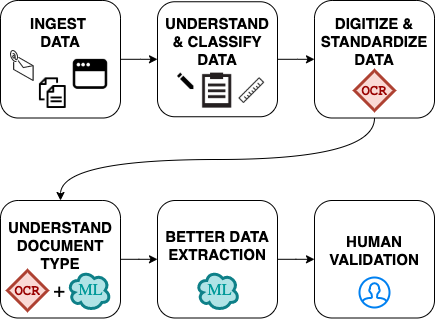
\includegraphics[width=\columnwidth]{HighLevelFlow.png}}
\caption{Document Flow in a Business Process}
\label{figHighLevelFlow}
\end{figure}

``Fig.~\ref{figHighLevelFlow}'' provides a high-level view of what it might look like to receive and handle files in a business process, whether automated or manual.

\subsection{Step 1: Ingest Data}
Depending on the business and the process involved, data can be received in a variety of ways. Customers may send emails with attachments or information in the body of the message. Files may be placed in a shared drive or submitted through a website dashboard. Smartphone applications might allow users to take a picture of the form and submit it for review.

\subsection{Step 2: Understand \& Classify Data}
These methods for receiving information can result in several file types that could be handled in different ways, depending on the data. We must find a method for understanding and classifying the data into one of three primary categories: Structured Data, Semi-Structured Data, and Unstructured Data.

\subsubsection{Structured Data}
Often in the format of comma-separated values (CSV) and spreadsheets, structured data is formatted in a consistent template. The page contains tables and predictable positions on the page or in the document.

This type of data can be gathered through simple data extraction scripts or template-based OCR. Rule-based approaches work well for this type of data.

\begin{figure}[ht]
\centerline{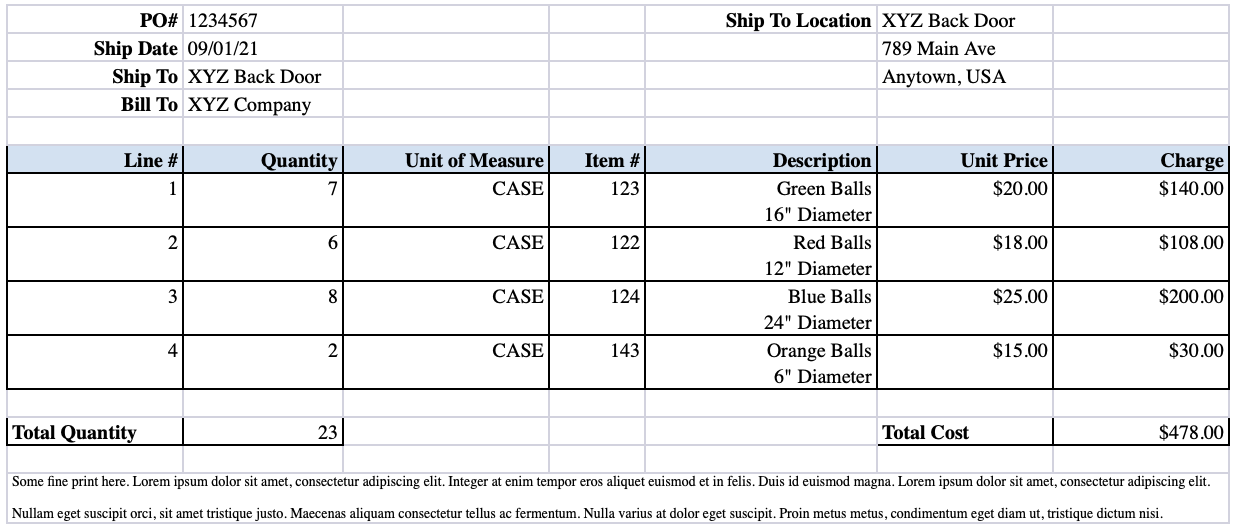
\includegraphics[width=\columnwidth]{Spreadsheet1.png}}
\caption{A templated spreadsheet for a purchase order.}
\label{figSpreadsheet1}
\end{figure}

If a business process involves receiving spreadsheets that are consistently structured like that in ``Fig.~\ref{figSpreadsheet1}'' allows for scripts to be written that can map using the expected position or with regular expressions to collect the data from the file. We've proven a sample of this in the simple Python code in Appendix A.

\begin{figure}[ht]
\centerline{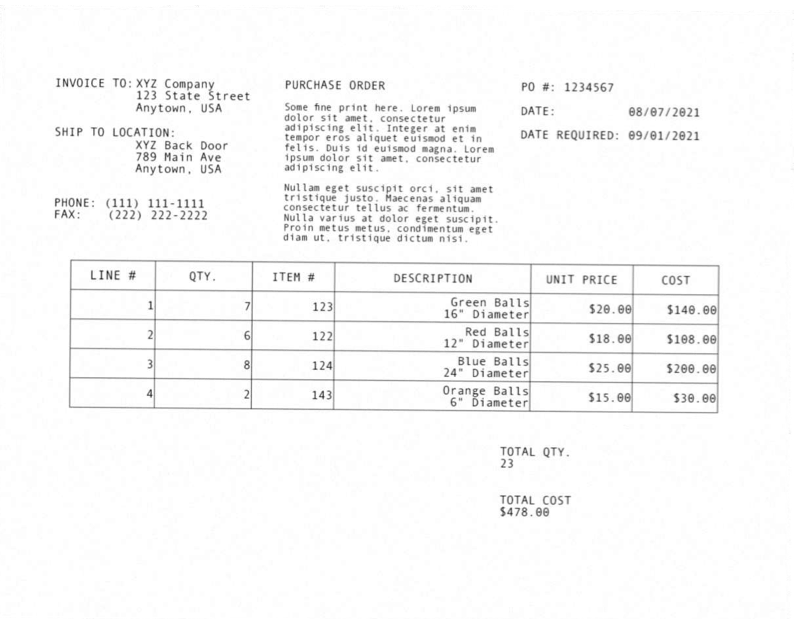
\includegraphics[width=\columnwidth]{ORDER_1_scanned.png}}
\caption{A templated scanned image for a purchase order.}
\label{figScanned1}
\end{figure}

Similarly, we might receive a scanned image of a purchase order that equally follows a template (like that in ``Fig.~\ref{figScanned1}''), but must be read using OCR. Processing the file through a basic OCR reader could provide us with a data structure similar to Appendix B, which can then be organized through additional scripts, though a bit more cumbersome to handle.

When templates maintain fixed positions and are consistent, understanding the data to classify it (separating purchase orders from invoices, etc) is generally straightforward.

\subsubsection{Semi-Structured Data}
However, if the template of the structured data isn't followed, the changes or variations require new rules. This might be a result of different regulations for a region requiring additional table columns in a purchase order, or larger customers using different systems that generate the files being provided.

\begin{figure}[ht]
\centerline{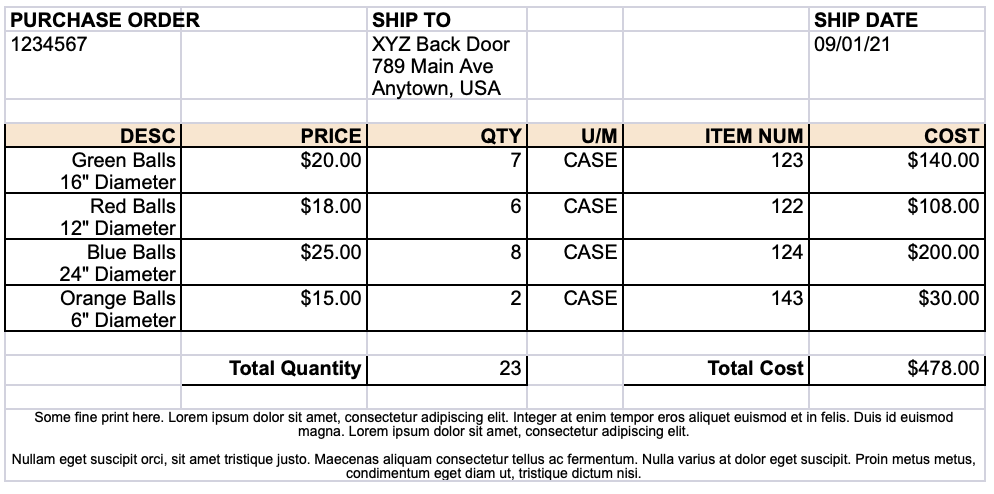
\includegraphics[width=\columnwidth]{Spreadsheet2.png}}
\caption{A templated spreadsheet for a purchase order containing the same information as ``Fig.~\ref{figSpreadsheet1}'', but with a different layout.}
\label{figSpreadsheet2}
\end{figure}

Documents that contain the same type of information but in different designs and layouts fall into the category of semi-structured data. The keys in key-value pairs are the same across all documents, but the position on the page might vary, as seen in Fig. 4. Similarly, we might see scanned images like Fig. 5 with varied layouts.

In this case, our rule-based approach gives us good accuracy for the document in ``Fig.~\ref{figSpreadsheet1}'', but low accuracy for the document in ``Fig.~\ref{figSpreadsheet2}''. If a business process is limited to only a few variations in the layout, writing a unique rule for each type is manageable. Appendix C provides additional code that can be applied to the same methods used in Appendix A that will work for the spreadsheet in ``Fig.~\ref{figSpreadsheet2}''.

However, this approach will have difficulty scaling for the semi-structured data. Companies will have to create a template creation and management process, adding and adjusting with each change and new layout.

Introducing automated intelligence (AI) at this stage can make it easier to scale at this stage of document classification and data extraction, avoiding template management, but introduces another layer of effort. Machine learning (ML), a specific form of AI, and deep learning models can assist in automatically detecting information desired from the input documents. Vihar Kurama suggests the use of several pre-trained ML models (FastRCNN, Attention OCR, and Graph Convolution) for a hybrid solution of both rules-based data extraction and ML \cite{kurama2021a}.

Important to note is that the reliance on automated extraction should always be kept in check by regular review of metrics, accuracy, and confidence scores. Thankfully the application of more samples to a machine learning model results in higher accuracy of the data retrieved.

\subsubsection{Unstructured Data}
The final classification for documents received would be unstructured data. This type of document has no key-value pairs, may contain handwritten text, is free-flowing, and lacks consistency.

Scripts and ML are not enough to understand and classify this data. Instead, we may need to consider other techniques, such as natural language processing (NLP). Another branch of artificial intelligence, NLP provides computers with the ability to understand the text of a document in the same way that human beings can \cite{ibm2020natural}.

\subsection{Step 3: Digitize \& Standardize Data}
With the process of understanding and classifying our data as structured, semi-structured, or unstructured, we now have some digital information that we can put to use. Our first pass at the documents might not have been deep enough to understand the document type; our business process may be more efficient at this point to gather just enough information to determine where to feed the document. By standardizing the data we've collected, we can continue to feed the documents through a pipeline.

\subsection{Step 4: Understand Document Types}
If our document ingestion receives a variety of document types, we need to now understand the document type. With the standardized data from the previous step, we should now be able to determine if the document is an invoice, a purchase order, an application, etc. Depending on the complexity of the business process involved, we may consider introducing machine learning in this step as well.

\subsection{Step 5: Better Data Extraction}
Once we know our document type (invoice vs. purchase order, etc.) we can now apply more specific data extraction methods. This may be more heavily focused on machine learning models if the documents are semi-structured.

This stage is a good placement for intelligent OCR. This is where model-based OCR engines can improve the process of digitizing the documents at scale while continuing to reduce errors with every training.

While many intelligent OCR tools are available, one such tool is the ABBYY FlexiCapture. In a review done by PricewaterhouseCoopers (PwC), ABBYY FlexiCapture was rated best in class in data validation and data classification, as well as data extraction in both structured and semi-structured documents. It also ranked well for multi-lingual capabilities, and the ability to read barcodes and tables. Google Tesseract and Microsoft's Modi ranked better for screenscraping in desktop, web, and documents. PwC goes on to note that ``the integration of the ABBYY OCR engine not only enhances automation for rules-driven processes, but also adds the flavour of NLP and widens the scope of automation.'' \cite{pwc2018robotic}

\subsection{Step 6: Human Validation}
While it's true that with machine learning we may need fewer human checks as we train with more samples, but a certain level of human-in-the-loop is necessary (and a good idea) when automating document handling. The continuous feed of more samples over time builds confidence in a process, but there should always be a human check to verify incoming information.

\section{Single Pipeline}
All of this has helped us understand the problem and an approach to handling documents. We have an idea of which types of tools might be useful and each particular step, but now we must understand how to string it all together into a single, cohesive pipeline.

A business process might begin as a simple macro or script, improving the time and effort needed for small tasks. From there, the process may see continued improvements through IT or business solutions. At some point, additional automation can be considered to raise the bar to another level: robotic process automation.

\subsection{Robotic Process Automation}
Robotic process automation, more commonly referred to as RPA, is the method of automating repetitive, often administrative, tasks. Generally speaking, virtual workers created for RPA will take advantage of a user interface on a screen, much like a human worker would do. These digital assistants will capture data and manipulate applications based on programmed decision-making. Similar to writing a programming script, RPA bots are made to mimic the same steps a human would do in particularly repetitive tasks, freeing up the human workers to focus on more valuable tasks.

In a survey of 100 document automation leaders by the Association of Intelligent Information Management, 18\% of the respondents use RPA and 12\% weren't sure of what RPA was. RPA with advanced capture has a place in the plans of 25\% of the respondents, but 42\% don't plan to make use of RPA. \cite{hollander2019survey}

Beyond standard RPA, where we automate the flow itself, we can level up again by using intelligent RPA, which leverages forms of artificial intelligence.

\begin{figure}[ht]
\centerline{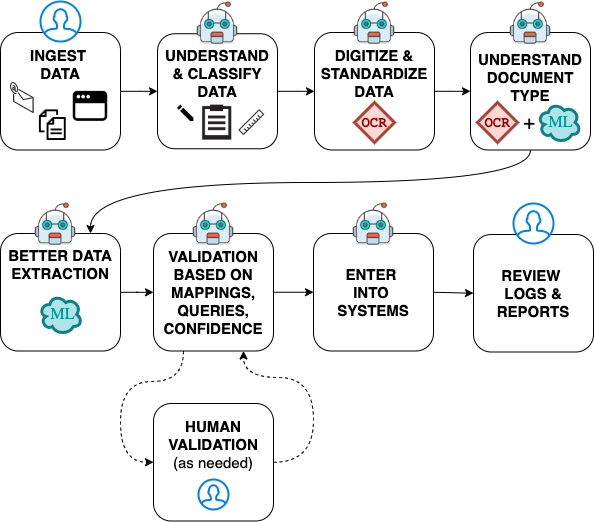
\includegraphics[width=\columnwidth]{BotFlow.png}}
\caption{Document Flow in a Business Process with RPA Bot and Human Worker ownership for each step.}
\label{figBotFlow}
\end{figure}

PepsiCo faced the challenge of a document processing flow that was slow, prone to errors, and very manual. When they applied a single process flow and involved the ABBYY FlexiCapture solution to their documents, they found that they had lower error rates, reduced processing times, and their Accounts Payable staff were able to work much more efficiently \cite{pepsico}.

Their flow is as follows:
\begin{enumerate}
\item Paper invoices (in any of 5 languages) are scanned locally
\item Scanned invoices are...
    \begin{enumerate}
        \item sent to the POWER Project
        \item identified with the correct entity
        \item recognized by FlexiCapture
    \end{enumerate}
\item New digital documents and data are sent to verification stations
\item Data is verified
\item Data is forwarded to PepsiCo's Image Vision for approval
\item Data is exported in XML
\item Data is processed in PepsiCo's SAP ERP solution
\end{enumerate}

``FlexiCapture's accuracy is also proving stable under a heavy workload. In its first three months the POWER Project solution has processed two thousand batches, over 21,000 documents and nearly 40,000 pages without issues – in a mix of five languages.'' \cite{pepsico}

This single pipeline solution has proven that it can scale and scale well!

\bibliographystyle{unsrt}
\bibliography{bibliography}

\onecolumn
\appendices

\newpage
\section{Python Methods to Collect Data from a Spreadsheet}
    \subsection{spreadsheets/methods.py}
    \lstinputlisting[language=Python]{Scripts/spreadsheets/methods.py}

    \newpage
    \subsection{spreadsheets/excel\_order\_one.py}
    These mappings are specific to the spreadsheet represented in ``Fig.~\ref{figSpreadsheet1}''.
    \lstinputlisting[language=Python]{Scripts/spreadsheets/excel_order_one.py}

\newpage
\section{Unit Tests for Python Methods in Appendix A}
    \subsection{tests/test\_spreadsheets\_methods.py}
    \lstinputlisting[language=Python]{Scripts/tests/test_spreadsheets_methods.py}

    \newpage
    \subsection{tests/test\_excel\_order\_one.py}
    \lstinputlisting[language=Python]{Scripts/tests/test_excel_order_one.py}

% \newpage
% \section{Data Collected as JSON from a Scanned Image}
% Below is a very small sampling of some lines at the beginning of a JSON file containing the data recognized from the scanned image (``Fig.~\ref{figScanned1}''):
% \lstinputlisting[linerange={1-29}]{Scripts/documents/OCRSpace_Order1.json}
% Below is a very small sampling of some lines at the end of a JSON file containing the data recognized from the scanned image (``Fig.~\ref{figScanned1}''):
% \lstinputlisting[linerange={1508-1519}]{Scripts/documents/OCRSpace_Order1.json}

\newpage
\section{Python Methods to Collect Data from a Spreadsheet}
    \subsection{spreadsheets/excel\_order\_two.py}
    These mappings are specific to the spreadsheet represented in ``Fig.~\ref{figSpreadsheet2}''.
    \lstinputlisting[language=Python]{Scripts/spreadsheets/excel_order_two.py}

\newpage
\section{Unit Tests for Python Mappings for Spreadsheet Order Two}
    \subsection{tests/test\_excel\_order\_two.py}
    \lstinputlisting[language=Python]{Scripts/tests/test_excel_order_two.py}

\end{document}
